\documentclass[border=6pt]{standalone}
\usepackage{fontspec}
\defaultfontfeatures{Ligatures=TeX}
\setmainfont{Palatino Linotype}
\usepackage{tikz}
\usetikzlibrary{arrows.meta, positioning, calc, shapes.geometric, fit,
                backgrounds, decorations.pathmorphing}
\definecolor{casink}{HTML}{1A1A22}
\definecolor{casaccent}{HTML}{6B3F8C}
\definecolor{casmuted}{HTML}{8A8A94}
\definecolor{caswash}{HTML}{F0ECF4}

\tikzset{
  casnode/.style={
    draw=casink, line width=0.5pt, rounded corners=1.2pt,
    fill=caswash, inner sep=3.2pt, font=\small, minimum height=6.5mm,
    align=center},
  casdomain/.style={
    casnode, minimum width=34mm, font=\small\bfseries},
  casflow/.style={
    -{Stealth[length=2.1mm,width=1.6mm]}, draw=casink, line width=0.55pt},
  casfeedback/.style={
    -{Stealth[length=2.1mm,width=1.6mm]}, draw=casmuted, line width=0.5pt,
    dashed, dash pattern=on 1.6pt off 1.4pt},
  casinvol/.style={
    {Stealth[length=1.8mm,width=1.4mm]}-{Stealth[length=1.8mm,width=1.4mm]},
    draw=casaccent, line width=0.5pt},
  caslabel/.style={font=\scriptsize, text=casmuted},
  cascap/.style={font=\scriptsize\itshape, text=casink},
}

% Every figure in this book uses the same wrapper so the list of figures and
% the numbering stay consistent.
\newcommand{\casfig}[3]{%
  \begin{figure}[htbp]
  \centering
  #2
  \caption{#3}\label{fig:#1}
  \end{figure}%
}

\begin{document}

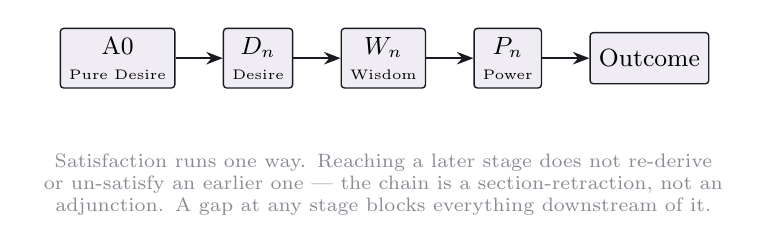
\begin{tikzpicture}[node distance=6mm]
  \node[casnode] (A0) {A0\\[-2pt]{\tiny Pure Desire}};
  \node[casnode, right=of A0] (D) {$D_n$\\[-2pt]{\tiny Desire}};
  \node[casnode, right=of D] (W) {$W_n$\\[-2pt]{\tiny Wisdom}};
  \node[casnode, right=of W] (P) {$P_n$\\[-2pt]{\tiny Power}};
  \node[casnode, right=of P] (O) {Outcome};
  \draw[casflow] (A0) -- (D);
  \draw[casflow] (D) -- (W);
  \draw[casflow] (W) -- (P);
  \draw[casflow] (P) -- (O);
  \node[caslabel, anchor=north, text width=88mm, align=center]
    at ($(W.south)+(0,-7mm)$)
    {Satisfaction runs one way. Reaching a later stage does not re-derive or
     un-satisfy an earlier one --- the chain is a section-retraction, not an
     adjunction. A gap at any stage blocks everything downstream of it.};
\end{tikzpicture}

\end{document}
